\documentclass[border=2pt]{standalone}
\usepackage{pgfplots}
\usetikzlibrary{plotmarks}
\pgfplotsset{compat=newest}
\begin{document}
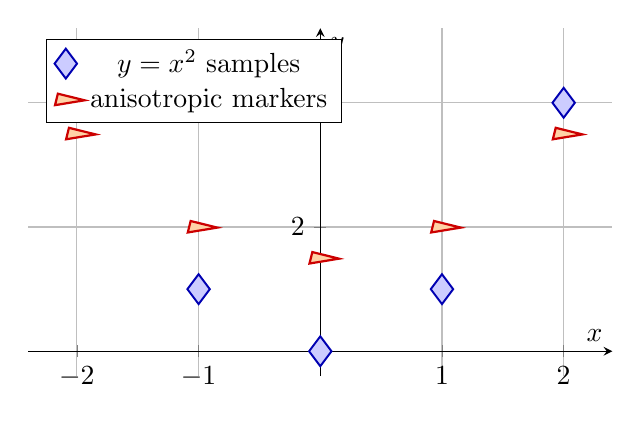
\begin{tikzpicture}
  \begin{axis}[
    width=9cm,height=6cm,
    xmin=-2.4,xmax=2.4,ymin=-.4,ymax=5.2,
    axis lines=middle,grid=major,
    xlabel={$x$},ylabel={$y$},
    legend pos=north west
  ]
    \addplot[only marks,mark=diamond*,mark size=4pt,
      every mark/.append style={scale=1.35,draw=blue!70!black,fill=blue!20,line width=.7pt}]
      coordinates {(-2,4) (-1,1) (0,0) (1,1) (2,4)};
    \addplot[only marks,mark=triangle*,mark size=4pt,
      mark options={xscale=1.7,yscale=.6,rotate=25,draw=red!80!black,fill=orange!35,line width=.8pt}]
      coordinates {(-2,3.5) (-1,2) (0,1.5) (1,2) (2,3.5)};
    \legend{$y=x^2$ samples,anisotropic markers}
  \end{axis}
\end{tikzpicture}
\end{document}
